\chapter{Systembeskrivelse}

Fra kundens synspunkt består systemet af en computer og nogle kontrollerbare stikdåser rundt i huset samt en babyalarm. Her beskrives hele systemet mere detaljeret.

\begin{figure}[H] \centering
\fbox{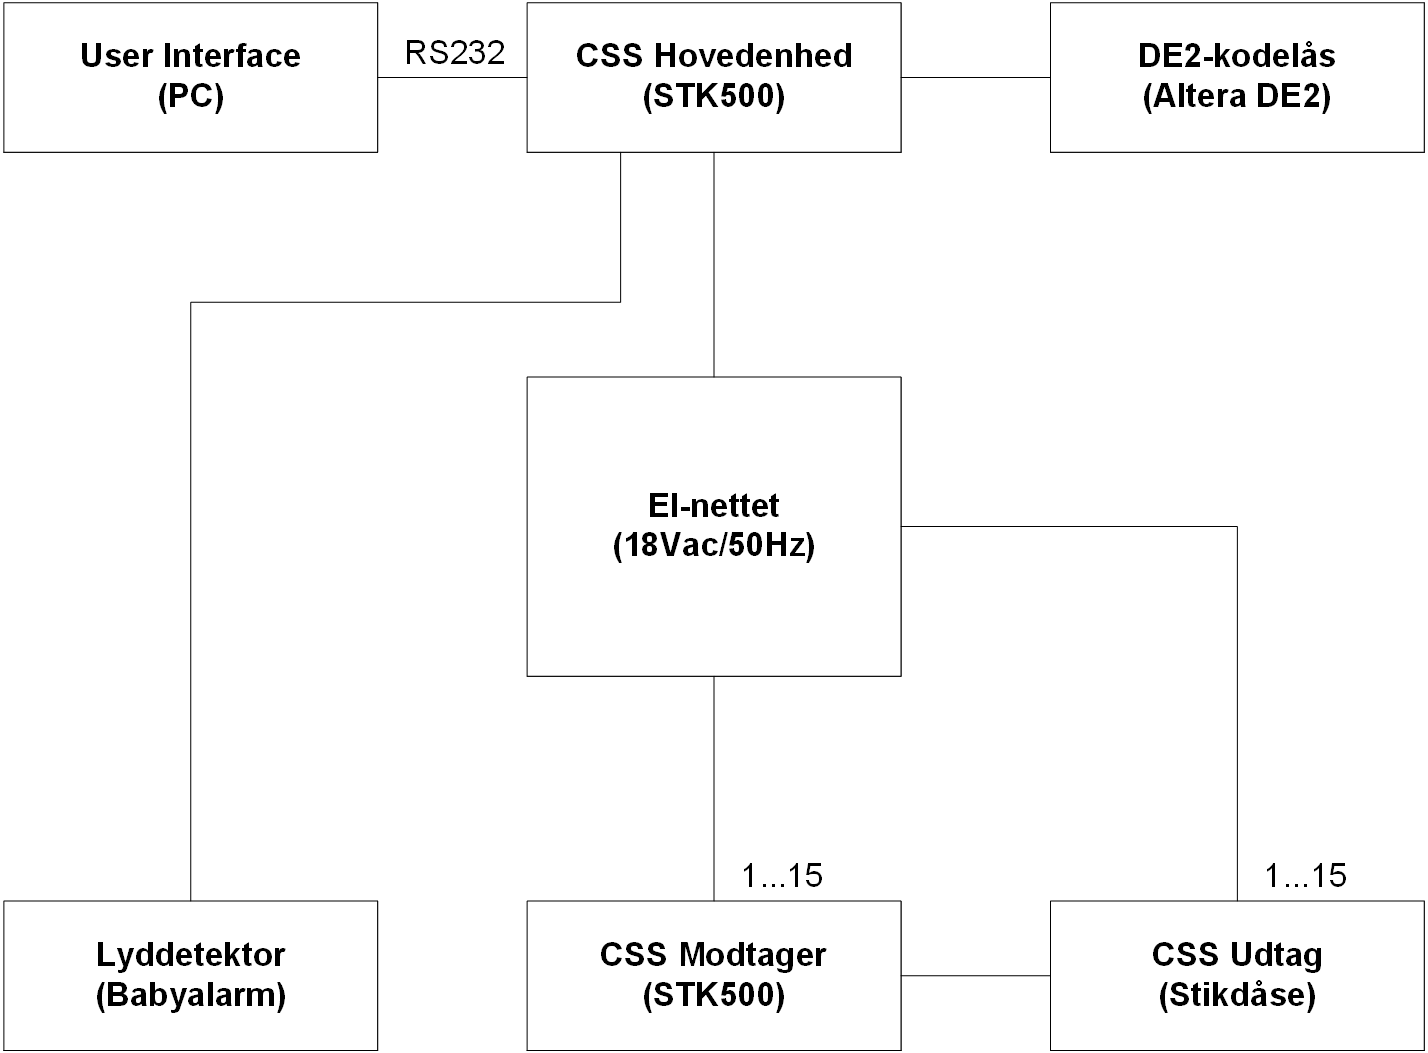
\includegraphics[width=0.65\textwidth]{billeder/diagrammer/Sys_oversigt}}
\caption{Systemoversigt}
\label{fig:sys_oversigt}
\end{figure}

I figur \ref{fig:sys_oversigt} ser man, at systemet består af en computer, der har forbindelse til CSS-hovedenheden; denne er kundens kontrolenhed(User Interface). Her har kunden adgang til et simpelt menusystem, hvori kunden kan kontrollere stikdåserne(CSS-udtagene). Der er mulighed for at aktivere, deaktivere eller udlæse status på systemet. Der er endvidere også mulighed for at ændre mobilnummeret til den person, som skal modtage babyalarm-SMS'en. Hele systemet kræver en 3 cifret adgangskode, der indtastes ved hjælp af et eksternt hardwaremodul(DE2-kodelås).

Når en kommando bliver eksekveret i User Interfacet, sendes der data serielt ud via RS232 til CSS-hovedenheden. Denne data bliver encodet til en X10-bitstrøm og sendt ud på el-nettet(18Vac). Denne bitstrøm bliver så aflæst af CSS-modtagerne, og hvis en CSS-modtager har den korrekte adresse, vil kommandoen blive udført på dens udtag. Et CSS-udtag kræver sin egen CSS-modtager.

Babyalarmens funktion er at give CSS-hovedenheden besked om støj i det værelse, hvor lyddetektoren sidder placeret. Lyddetektoren er kablet direkte til CSS-hovedenheden og virker ved, at den ved et givent lydniveau\footnote{se ikke-funktionelle krav i produktdokumentationen} vil sende et signal til CSS-hovedenheden, som via dennes serielle port fortæller PCen, at der skal sendes en SMS til det forudbestemte mobilnummer med en advarsel.

\subsection*{Installation i hjemmet}

Her ses, hvordan installationen kunne laves i en kundes hjem. Hængelåsene angiver hvilke enheder i hjemmet, der kan interageres med.

\begin{figure}[H] \centering
\fbox{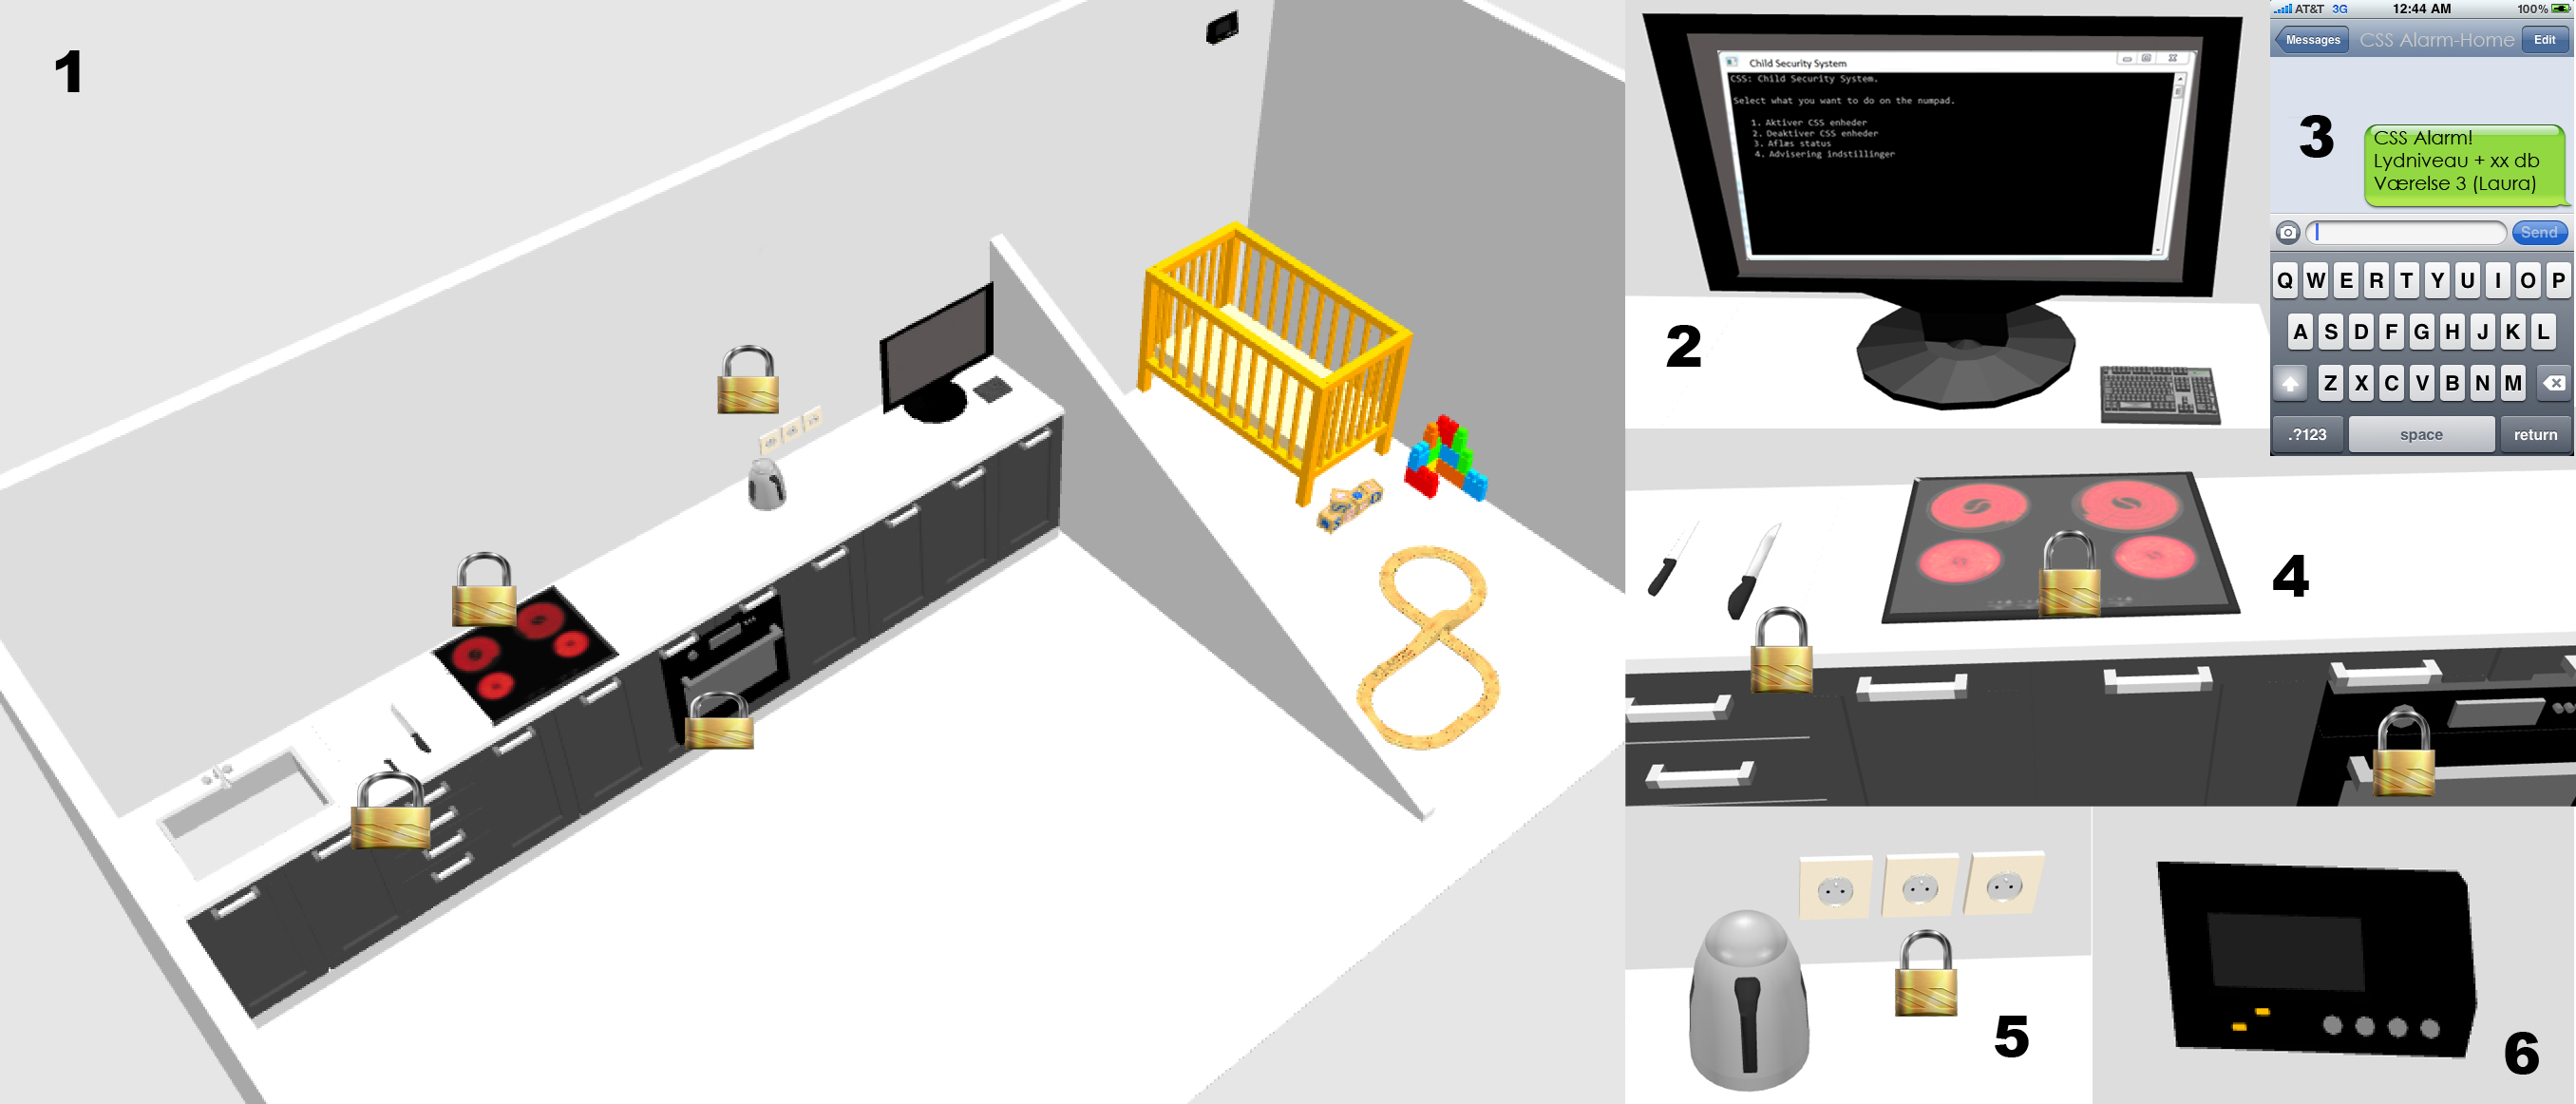
\includegraphics[width=0.65\textwidth]{billeder/Installationsoversigt}}
\caption{Installationsoversigt}
\label{fig:installationsoversigt}
\end{figure}

\begin{enumerate}
\item Samlet oversigtstegning af CSS. 
\item CSS-programmet med tilhørende DE2-kodelås.
\item SMS-besked udsendt af systemet, idet lydniveauet i værelse 3 (Laura) har været over det tilladte.
\item Overblik over, hvad systemet er tiltænkt at børnesikre. Køkken skuffe med skarpe genstande, kogeplader, ovn.
\item 230V udtag. X10 styret, således at det bestemmes, om udtaget skal være aktivt.
\item Babyalarm. Illustrationen vil variere i forhold til virkeligheden.
\end{enumerate}